% !TEX root = ../Yan Hao--Dissertation.tex

\chapter{Intergovernmental Transfer Decision: an Outcome of the Interaction between Central and Local Government}


\section{Introduction}

Fiscal federalism is essential for optimizing the delivery of public goods and services, leveraging local governments' unique insights into community needs  \parencite{hayek2009use,stigler1998tenable}. Central to this system are intergovernmental transfers, which facilitate collaboration between central and subnational governments, ensuring efficient provision of public services  \parencite{press1963american, grodzins1966american}. Despite the recognized benefits of such decentralization, the intricacies of policy outcomes stemming from intergovernmental interactions are not fully understood.

Despite scholarly consensus on the interactive nature of transfer payment formation, the precise mechanisms governing the selection and distribution of transfer payment tools, particularly within the context of the United States, remain elusive \parencite{1988Exploring,1967American, 2010Centralization,chubb1985political,1976A,dixit1995redistributive}. The lack of understanding of the mechanism for selecting fiscal tools has led to a limited comprehension of certain fiscal phenomena. For instance, the predominance of categorical transfers, comprising approximately 80\% of total transfer payments in the United States, raises questions about the underlying factors driving this distribution imbalance \parencite{dilger2015federal}.


This chapter introduces a study that aims to bridge the knowledge gaps identified earlier, specifically regarding the decision-making processes guiding the selection of intergovernmental transfer tools and the fiscal phenomena inherent in the transfer payment process. First, it seeks to uncover the decision-making processes guiding the selection of intergovernmental transfer tools. Second, it endeavors to elucidate fiscal phenomena inherent in the transfer payment process, including the flypaper effect, differential impact of direct government involvement versus transferring grants to local governments, and the prevalence of categorical transfer. Grounded in game theory, this study endeavors to provide insights into these fiscal phenomena and contribute to a deeper understanding of the forming mechanism surrounding intergovernmental transfers.


%%%%%%%%%%%%%%%%%%%%%%%%%%%%%%%%%%%significance%%%%%%%%%%%%%%%
In this chapter,I explore the strategic interactions between central and local governments within fiscal federalism, providing both theoretical insights and empirical evidence. Building on the dissertation's objectives outlined in Chapter 1, this part focuses on how these interactions influence fiscal policy decisions and their implications for public goods provision. By investigating the decision-making mechanisms behind intergovernmental transfers, this chapter offers insights into the fiscal dynamics between governmental tiers, crucial for both theoretical understanding and policy design.

This analysis not only contributes to the academic discourse on fiscal federalism but also guides policymakers in enhancing fiscal collaboration between government levels. Highlighting methodological innovation, the chapter aims to deepen the comprehension of fiscal behaviors across government tiers, directly impacting the design of efficient and equitable fiscal transfer mechanisms.

Summarily, this chapter is integral to the dissertation's aim of examining the complex fiscal interactions under fiscal federalism and lays foundational work for the concluding synthesis of findings


%%%%%%%%%%%%%%%%%%%%%%%%%%%%%%%%%%%
The forthcoming sections are organized as follows: Initially, a comprehensive background sets the stage, delving into the intricacies of intergovernmental transfer policies. This is followed by a critical literature review, which lays the groundwork by discussing existing theories and identifying gaps this study aims to fill. Subsequently, the method section outlines the construction of the game theory model, detailing its components such as player set, action set, and utility set. The model solving procedure then elucidates the application of backward induction to derive theoretical implications. Results are presented, highlighting the implications of different transfer mechanisms on public goods provision and intergovernmental transfer choices. Finally, the paper concludes with a review and summary, reflecting on the study's contributions to the understanding of fiscal federalism and intergovernmental transfers.

\section{Background}

This section elucidates the interaction between national and subnational governments in formulating intergovernmental transfer policies within actual administrative processes. Following \textcite{volden2007intergovernmental}, the grant-making process encompasses four interrelated decisions. Initially, the national government assesses its participation in subnational public goods provision. Upon deciding to engage, it then determines the modality of support for subnational jurisdictions. Common approaches include direct provision, termed as joint provision, and the issuance of intergovernmental grants. These methods are delineated as follows:

\begin{itemize}
    \item \textbf{Joint Provision}
\end{itemize}

Here, the national government actively participates in delivering public goods alongside subnational entities. An illustrative example is the collaboration between the United States Department of Labor and subnational governments in administering labor training and rights protection programs, such as the Veterans' Employment and Training Service (VETS) and the Wage and Hour Division (WHD).

\begin{itemize}
    \item \textbf{Intergovernmental Grants}
\end{itemize}


These grants vary by their allocation mechanisms, encompassing project grants, formula grants, and reimbursement grants. Project grants are competitively awarded, promoting innovative projects at the state level. Formula grants are distributed based on predefined criteria that reflect the social characteristics of jurisdictions\parencite{huffman2006formula}. Reimbursement grants, either open-ended or closed-ended, compensate state and local governments for specific program expenditures.


Subsequent to the grant allocation mechanism determination, local governments decide on grant acceptance and the application of funds. These sequential decisions culminate in the formulation of public goods provision policy, positioning the national government as either a direct provider, a facilitator through grants, or a non-participant in subnational initiatives.


\section{Problem Statement}
The central problem addressed in this article is to unravel the complexities underlying the formation of fiscal policies governing transfer payments. Contrary to the perception of a straightforward top-down approach, the consensus among scholars suggests that fiscal policy outcomes represent a negotiated compromise across governmental tiers\parencite{chubb1985political, 1976A, dixit1995redistributive}. Yet, the detailed mechanics of policy tool formulation—encompassing evaluative considerations, sacrifices, and compromises between central and local governments—remain insufficiently integrated into a cohesive analytical framework. This article is particularly concerned with the rationale behind the preferential selection of specific transfer payment instruments and the reasons underlying the disproportionately high reliance on categorical transfers, which account for about 80\% of all transfer payments in the United States\parencite{dilger2015federal}. How can we explain this highly unbalanced distribution of transfer payments?

The research questions guiding this investigation are twofold:
\begin{itemize}
    \item Mechanism of Intergovernmental Transfer Tool Determination.
\end{itemize}

This study seeks to demystify the process governing the selection of transfer payment instruments, aiming to elucidate the criteria and considerations driving this choice.

\begin{itemize}
    \item Examination of Fiscal Phenomena within Transfer Payments.
\end{itemize}

Leveraging a theoretical framework, the article aims to shed light on fiscal phenomena observed in the transfer payment process, including the flypaper effect and the differential impact of direct government provision versus grant transfers on local public goods provision. A particular focus is placed on explaining the pronounced preference for categorical transfers within the United States.

Through addressing these inquiries, the article endeavors to contribute to the scholarly understanding of fiscal policy formation in intergovernmental transfers, offering theoretical insights into observed fiscal behaviors and policy preferences.

\section{Literature Review}
This literature review is structured around \textcite{volden2007intergovernmental}'s analytical framework, which delineates the interaction between national and subnational governments in the context of fiscal federalism into four distinct categories. By dissecting the literature according to this schema, this review explores the multifaceted factors influencing the patterns of interaction between different levels of government and identifies areas where this study can make a substantive contribution. The framework begins by examining the central government's role in the first two steps, focusing on the formulation and decision-making processes regarding grants-in-aid. It then transitions to the subnational perspective in the latter two steps, scrutinizing local governments' responses to federal decisions and their strategies for public goods provision. Throughout, this review emphasizes the interplay between national and subnational entities, shedding light on the nuanced dynamics that characterize fiscal federalism.

\subsection{On National Government Level}

The allocation of grants at the central government level is often conceptualized as a strategic bargaining game among key decision-making entities, such as committees, congress, or legislative houses. The seminal work of \Textcite{baron1989bargaining} introduced foundational assumptions to the study of these bargaining processes, including random recognition, majority voting rules, and earmarking practices.  They made several important assumptions, such as random recognition, majority voting rule, and earmarks rule. Their analysis, further generalized by \Textcite{banks2006general},elucidates how legislators possessing agenda-setting capabilities tend to secure a disproportionate allocation of funds. In a significant development,  \Textcite{martin2018dividing} nuances this view by limiting the scope of decision-makers to influence only the criteria of funding distribution, not the exact allocations, thereby more accurately mirroring the intricacies of political and administrative decision-making. Contrary to earlier models, Martin's findings suggest the formation of oversized coalitions and the emergence of stable winning groups.

Except for the theoretical investigation of the decision making bargaining process, scholars also focus on the empirical evidence of the impact of some socio-economic factors on grants-in-aid distribution. \Textcite{markusen1981benefits} explored temporal shifts in federal grant allocations to cities across different regions during the 1960s and 1970s, uncovering significant increases and regional variations in funding patterns that align with shifts in political landscapes. Similarly, \Textcite{wallis1987employment} and \Textcite{stegarescu2006decentralised} highlight the political and demographic factors influencing intergovernmental transfers, with Stegarescu pointing to the role of population size, unemployment rates, openness to trade, and political systems in determining the extent of fiscal decentralization.  \Textcite{kasdin2016decision} adds to this discourse by illustrating how the network complexity of state or local governance structures can affect both the volume of federal transfers and the degree of federal oversight, emphasizing the pivotal role of governance networks in shaping fiscal federalism.

This body of literature, focusing primarily on the initial stages of Volden's framework, underscores the multifaceted nature of grant distribution at the national level, revealing a complex interplay of strategic bargaining, socio-economic factors, and political dynamics.

\subsection{On Subnational Government Level}

Volden's framework's concluding phases delve into the realm of local governance, examining how subnational entities respond to federal initiatives and the resultant implications for local spending strategies. This segment of literature underscores the nuanced deliberations local governments undertake when navigating grant opportunities, influenced significantly by political dynamics and fiscal policies.

\Textcite{nicholson2012leaving} d highlights how partisan and electoral pressures significantly shape state-level grant applications, suggesting a strategic calculus behind the acceptance or rejection of federal grants. Complementarily, \Textcite{volden2005intergovernmental} explores the competitive dynamics between central and local governments over public goods provision, positing that local governments may control the scale of transfer payments received within their jurisdiction due to potentially greater political leverage.
%%%%%%%tag
The discourse on the fiscal impact of intergovernmental transfers (IGT) on local government spending is both broad and deep. \textcite{pack1993foreign}introduce the concept of "fungibility," proposing that local governments might use federal funds to supplant their revenue streams, thereby altering spending patterns on public goods and local taxation. Despite its intuitive appeal, empirical support for this notion remains sparse.

In contrast, the "flypaper effect" garners substantial empirical backing \parencite{hines1995anomalies,gamkhar2007impact}.  This theory, articulated by  \textcite{bradford1971analysis}, posits that federal grants have a more potent effect on local spending than equivalent increases in local revenue, challenging the equivalence theorem predicated on the median voter theorem and lump-sum tax collection. However, empirical evidence does not support this theorem. Specifically, some researchers have found that a $1$ increase in individual revenue leads to an increase in public expenditure of only $0.02$ to $0.05$, while a $1$ increase in intergovernmental transfers can lead to an increase in public expenditure of $0.25$ to even $1$ \parencite{bailey1998flypaper,dollery1996empirical,gamkhar2007impact}. This counterintuitive outcome, extensively documented in over 3500 studies as noted by \Textcite{inman2008flypaper}'s statistics, underscores the unique influence of federal grants on local fiscal behaviors.


\subsection{My Rethinking of the Literature}
\Textcite{volden2007intergovernmental} makes a seminal contribution by developing a game theory framework that intricately links the decision-making processes across government levels in the context of intergovernmental transfers. His model provides a systematic mechanism for understanding the flow of funds from central to local governments. However, the model faces challenges, particularly regarding assumptions about voter information and the scope of transfer tools.

\subsubsection{Revisiting Voter Information Assumptions}
Volden's model presupposes that voters have the capacity to discern the origins of public goods and the allocation of tax burdens, enabling them to assign political credit accurately. This assumption hinges on the notion that voters possess comprehensive information about spending and can attribute credit for public goods provision proportionally \parencite{volden2005intergovernmental}. The assertion that voters accurately ascribe electoral credit and blame is primarily based on a federalist perspective on vote choice \parencite{stein1990economic}. Some earlier empirical literature supports this assumption \parencite{atkeson1995economic}. There is empirical evidence, however, showing that at least in America, voters inaccurately ascribe credit and blame for public goods provision. Studies by \Textcite{carpini1996americans} demonstrates that only 14\% of the interviewees are aware of the unemployment rates, and 25\% knew about the proportion of federal spending in terms of education resource supply. Additionally, \Textcite{gilens2001political} indicates that only 12\% of the respondents provided correct answers regarding whether the crime rate has risen or declined in the last decade. Needless to say, a substantial body of literature on fiscal illusion, discussing voters' inaccurate sense of the price of public goods, also serves as strong evidence of voters' insufficient information \parencite{oates1979lump,borge1995lump,turnbull1998overspending}. This body of work underscores the complexities of voter knowledge, challenging the assumption of informed electorate decision-making.

\subsubsection{Expanding the Transfer Toolset}
Another critique centers on the model's limited consideration of transfer mechanisms, focusing predominantly on general transfers and overlooking the nuanced role of categorical grants. Given the substantial portion of grant funding categorical transfers represent, especially in policy adjustments, their exclusion narrows the model's applicability. This paper proposes to broaden the framework to include a more diverse array of transfer instruments, thereby enhancing its relevance and utility.

To address these gaps, this study introduces modifications within a complete information dynamic game framework. It incorporates fiscal illusion considerations, particularly the impact of transparency in public goods provision versus tax collection. Recognizing the differential clarity between these two processes acknowledges the real-world complexities of fiscal federalism. Public goods provision involves more institutions and layers of government compared to tax collection. \Textcite{bednar2007credit} argue that once the level of public goods provision reaches a certain threshold, citizens become indifferent to the supplier of the goods. Similarly, \Textcite{nicholson2011claiming} contend that the political credit derived from public goods provision lacks a clear assignment. Tax collection, on the other hand, is directly linked to the general public, allowing taxpayers to have a clear understanding of the amount of tax collected by various levels of government.To summarize, public goods provision process is less transparent compared to tax collection \parencite{mcgillivray2019aid,pommerehne1978fiscal, cepparulo2019public}.

The expanded model also includes categorical transfers, reflecting a more comprehensive array of tools at the disposal of the central government. This adjustment allows for a richer analysis of policy dynamics and the strategic considerations underpinning intergovernmental fiscal relationships.

By integrating these modifications, the paper not only critiques and builds upon Volden's foundational framework but also offers new insights into the intricacies of fiscal federalism, with a particular focus on the roles of transparency, voter information, and the diversity of transfer mechanisms.


\section{Method}
The theoretical framework is built upon a dynamic game model with complete information. The theoretical implications are derived through backward induction. Following the solution of the game theory model, I will utilize the theoretical implications to elucidate certain fiscal phenomena in intergovernmental transfers.


\subsection{Game Theory Model Construction}

Building upon \Textcite{volden2007intergovernmental}'s dynamic game framework, I formulated my own dynamic model. The game is structured as a dynamic game with complete information, signifying that the utility for all players in this game is common knowledge. The model construction can be delineated from three aspects: players in the game, available behaviors for the players, and utility for the players.

\subsubsection{Player Set}

Three players participate in this intergovernmental transfer game: the central government $N$\label{player}, state governments with higher resource endowment $S_h$, and state governments with lower resource endowment $S_l$. The assumption of identical subnational governments in Volden's paper is relaxed. Governments with different resource endowments may have varying fiscal preferences, leading to distinct reactions to intergovernmental fiscal policy. The player set can be defined as $P = { N, S_h, S_l}$. For convenience, I denote $i\in {l,h}$, where the difference between $S_h$ and $S_l$ lies in the fact that states with higher resource endowments are more productive and possess higher tax bases (GDP). Thus, I have $F_h>F_l$.%%corrected by chatgpt

\subsubsection{Action Set}
I summary the available action for national government and subnational governments separately.

\begin{itemize}
    \item \textbf{Action set summary for national government}
\end{itemize}

For the central or national government, one available option is to refrain from participating in the subnational jurisdictions' public goods provision. I refer to this subgame as the "no provision" game. Alternatively, if the national government decides to engage in provision, the next question is how to participate. The available choices include the joint provision game, general transfer game, or categorical transfer game.

In the joint provision game, the national government provides the goods directly. In this scenario, citizens in a specific $S_i$ benefit from the public goods offered by both national and subnational governments combined. In the joint provision game, the national government is the direct provider of the goods and determines the amount of public goods provided to $S_i$, denoted as $G_{Ni}$.%%%corrected by chatgpt

Another subgame involves offering intergovernmental transfers. In Volden's framework, the national government can provide grants only through general transfers, which are lump-sum subsidies. I assume there are two types of intergovernmental transfers. Transfers to lower-level governments are either general transfers ($GT$)\label{transfer} or categorical transfers ($CT$). $CT$ is more restricted during the spending process, and subnational governments cannot use the grants freely as they wish. As shown in Table \ref{Table 1.3}, highly restricted grants are only allowed to be spent in specific areas. Volden didn't distinguish between different types of grants in his dynamic game setting. However, the restrictions may play a role in influencing both national and subnational governments' behavior.


The motivation for the national government to choose between general transfer and categorical transfer is different. The primary goal of the national government in participating in the general transfer subgame is to narrow the utility gap of $S_i$ and equalize the original resource endowment difference. The effects of general transfer have been widely discussed in fiscal federalism literature \parencite{buettner2006incentive,lv2018transfer}. On the other hand, categorical transfer is employed to achieve specific political goals. For instance, the national government may aim to stimulate spending in a particular area.Therefore, differentiating between general transfers and categorical transfers is quite necessary.

I adopted \Textcite{buettner2006incentive}'s design about the amount of general transfer, in which general transfer amount $T$ received by government $i$ can be captured as:

\begin{equation}
    T_i = T_0 - \sigma F_i\label{generaltransfer}
\end{equation}


where $\sigma$ captures the central government's subjective intention to equalize resources in different jurisdictions. A higher $\sigma$ indicates that the national government prefers to equalize resources. For example, compared to the US federal government, OECD central governments may prefer to set a higher $\sigma$. $T_0$ is the benchmark grant amount when $S_i$ has zero $F_i$. $F_i$ is the total production output, which is also the tax base of $S_i$.


Compared to general transfers, equity is not a primary concern in the categorical transfer game. The role of categorical grants is to influence policy direction in subnational jurisdictions. By encouraging spending in a specific area, the central government could steer policy output in a nationally favored direction. Categorical transfers are typically matching transfers, where the national government covers a specific percentage of expenditure in a particular area, and subnational governments cover the rest. I assume there are two types of public goods at the subnational level: productive goods ($P$), such as roads, railways, and other types of infrastructure, and welfare public goods ($W$), such as social welfare and salaries for public servants.%%%chatgpt checked


In the categorical transfer game, I assume the matching ratio for productive grants is $m$\label{generalandcategorical}, and the matching ratio for welfare-oriented grants is $n$. Thus, the productive and welfare-oriented grants received by subnational government $i$ are:

\begin{equation}
    \left\{\begin{array}{l}
        T_p^i=m P_i \\
        T_w^i=n W_i
    \end{array}\right.\label{mrmatrix}
\end{equation}

To summary, the available action for national government is $$A_N=\left\{N P,\left(J P, G_{Ni}\right),\left(G T, T_0, \sigma\right),(C T, m,n)\right\} $$

\begin{itemize}
    \item \textbf{Action set summary for subnational governments}
\end{itemize}

For subnational governments, they need to decide on the public goods $G_i|{NP}$ they provide under the no provision game, the public goods they provide $G{si}|{JP}$ under the joint provision game, and the public goods $G_i|{GT}$ under the general transfer game. I assume subnational governments cannot reject joint provision or general transfer since joint provision and general transfer are lump-sum supplements. For categorical grants, I assume subnational governments may choose to reject based on their utility considerations. If subnational governments choose to reject the grants, then the national government is out of the game, and the game becomes a no provision game. If subnational governments decide to accept the grants, then they need to decide the amount of public goods they provide $G_i|_{CT}$ based on the matching ratios $m$ and $n$ offered by the national government. To summarize, the action set for subnational governments $A_i$ \label{action} is:

$$A_i=\left\{\left(G_i|_{NP}\right),\left(G_{si}|_{JP} \right),\left(G_i|_{GT} \right),\left(Accept,G_i|_{CT}\right), (Reject,G_i|_{NP})\right\} $$

\subsubsection{Utility Set}

I followed the design of Volden's design but with multiple new considerations. The utility of national government and subnational governments are also summarized separately.
\begin{itemize}
    \item \textbf{Utility for subnational government}
\end{itemize}

For subnational governments, the utility function can be listed as:

\begin{equation}
    U_i=\alpha_i G_i-t_{i}^2\cdot f_i-\gamma_i\left|y_i-X_i\right|
\end{equation}

I set $G$ as  Cobb-Douglas form public goods utility compound affected by the amount of $P$ and $W$.

\begin{equation}
    G_i= P^{\beta_i} W^{\epsilon_i}\label{pgmatrix}
\end{equation}

$\alpha_i$ is the marginal utility of $G_i$, which could be explained as the scarcity level of the public goods in place $i$. $\beta_i$ and $\epsilon_i$ are elasticity of productive public goods and welfare public goods and I assume $\beta_i + \epsilon_i<1 $ since part of the utility also comes from private goods consumption.


The utility for subnational governments comprises three components. Firstly, there is utility derived from the provision of public goods, denoted as $G$. Secondly, the tax burden, represented by $t_i$ and imposed by both national and subnational authorities, injures the overall utility. The quadratic form of the tax burden reflects the risk-averse disposition of the citizens.

The fraction factor $f_i$ signifies the proportion of blame attributed to the subnational government for tax increases, expressed as $f_i=\frac{t_i}{t_i+t_N}$. It is crucial to note that there is no analogous fraction factor for the credit associated with supplying public goods. This omission accounts for the observation that subnational governments receive full political credit for any augmentation in public goods, regardless of whether the goods are supplied by the national government.%%%%checked by chatgpt already


The third segment delineates the policy direction, compressing it into a one-dimensional continuum represented by $X_N$ and $X_i$" on opposing ends. The actual policy outcome in jurisdiction $i$, denoted as $y_i$, resides between these two end points. Each government entity possesses an ideal policy outcome denoted by $X_N$ and $X_i$. The disparity between the actual policy outcome and the ideal outcome for jurisdiction $i$, expressed as $|y_i-X_i|$, signifies the influence of both national and subnational factors on policy direction.

The rationale behind $|y-X_i|$ \label{actposition}lies in capturing the policy distance, elucidating the divergence between the actual and ideal policy outcomes. Additionally, a parameter $0<\gamma_i\leq 1$ is introduced, with $\gamma_i|X_N-X_i|=|y_i-X_i|$. This term encapsulates the "alliance effect," reflecting potential collaboration or alignment between national and subnational governments. The parameter $\gamma_i$ assumes a minimum value when shared ideologies exist between the two levels of government. In cases where federal and state governments occupy polarized positions, $\gamma_i=1$, indicating a lack of alignment. In this scenario, there exists a maximum distance between the actual policy outcome and the ideal policy point.%checked by chatgpt


% The third part captures the policy direction. I compress the policy direction to a 1 dimension line with $X_N$ and $X_i$ on two sides. The actual policy outcome lies in somewhere between $X_N$ and $X_i$. Each government has an ideal policy outcome point on a one dimensional line. $y$ is the actual policy outcome and $X_i$ means the ideal policy outcome for jurisdiction $i$. $|y_i-X_i|$ captures the distance between the actual policy outcome and the ideal policy outcome of $S_i$. The logic of this term is that the policy direction is typically an outcome of both national and subnational impact. For example, central government prefer the policy direction with less negative externality while subnational government focus merely on their own benefits.\label{iposition} While $|y-X_i|$ expresses the policy distance. Besides,I add a $0<\gamma_i\leq 1$ and let $\gamma_i|X_N-X_i|=|y_i-X_i|$ to capture the possible "alliance effect". For example, for specific policy gap between national and subnational governments, national governments may have preference on a specific jurisdiction $S_i$, or subnational government may take a lower threshold to accept the restriction if national government and a specific subnational government are alligned. $\gamma_i$ may take a minimal value when national government and subnational government share similar ideas. If federal and state governments stand in polarized opposite position, then $\gamma_i=1$ \label{actposition}.

Essentially, subnational governments seek to maximize the utility derived from public goods while managing the attribution of tax burden blame from citizens and exerting control over the policy outcome in accordance with their policy preferences.

\begin{itemize}
    \item \textbf{Utility for national government}
\end{itemize}

For national government, the utility function can be listed as:

\begin{equation}
    U_N = \sum_i \alpha_i G_i - \sum_i (t_{Ni}+t_{si})^2\cdot \frac{t_{Ni}}{t_{Ni}+t_{si}} - \sum_i \gamma_i |X_i-X_N| \label{utilityforng}
\end{equation}


The utility for the national government comprises three components\footnote{The utility calculation for the national government differs slightly from that in Equation \ref{utilityforng}. I assume the national government issues bonds to collect revenue rather than relying on taxes. This will be elaborated upon in detail later.}.  Firstly, the national government is concerned with the utility derived from increasing public goods across all subnational jurisdictions. The second term encapsulates the tax burden attributed to the national government. The third term expresses the utility derived from a policy direction favorable to the national government.%chatgpt checked


\Textcite{volden2007intergovernmental}'s balanced budget assumption continues to apply to both national and subnational governments in this paper. This implies that all tax income is invested in public goods provision. Let $c_i$ denote the price for public goods in jurisdiction $i$, and $e_j$ represent the tax collection efficiency of player $j \in P$. The efficiency $e_j$ is influenced by various factors such as the number of administrators, salary levels within the tax administration system, and IT expenditure on equipment \parencite{savic2015impact, kiser1994could, aizenman2008collection, mattos2011flypaper}. Additionally, subjective attitudes, such as the effort exerted by the government in tax collection, also impact $e_j$.

Under the balanced budget assumption, the equation $\frac{c_i G_s^i}{e_i F_i}=t_i$ holds at the subnational level.\label{priceandeffort}

Based on the construction of the game, the interaction process can be listed as figure \ref{dynamicgamenoutility}.

% \newpage
% % \begin{landscape}
% \begin{figure}[H]
%   \centering
%   \includegraphics[scale=0.045]{Chapter-2/Figures/tree.jpg}
%   \caption[Dynamic Game Tree of 3 players]{Dynamic Game Tree between Central and Subnational Governments
%     \texttt{} }
%   \label{dynamicgamenoutility}
% \end{figure}
% % \end{landscape}
% \newpage

\section{Model Solving Procedure}

The game is solved through backward induction. Initially, subnational governments compare their utility under each subgame and decide whether to accept the offer based on this utility\footnote{Since subnational governments have no incentive to reject the national government's joint provision and general transfer decision, the utility of subnational governments in the joint provision and general transfer subgame is irrelevant and is therefore not included in the table.}. As this is a complete information game, the national government knows the utility of the subnational government. Subsequently, the national government calculates its own utility based on the choices made by the subnational governments.

To solve the game theory model, the process starts from the tail end of the branch, systematically computing the utility of both subnational and national governments under each subgame.%%%%%chatgpt checked

\subsection{No Provision Game}

Under the no provision game, the subnational government is the sole provider of public goods. In this game, utility is determined by the quantities supplied by the subnational government. Additionally, the subnational government bears the entire responsibility for raising the required taxes. Finally, in this game, the subnational government exclusively determines the policy outcome, hence $y_i=X_i$. In this scenario, the utility of subnational governments is expressed as:

\begin{equation}
    U_i=\alpha_i G_i-\left(\frac{c_i}{e_i F_i} G_i\right)^2 \label{utilityforsi}
\end{equation}

where $c_i$ is the price for the public goods compound.

Equation \ref{utilityforsi} can also be written in $P$ and $W$ as:

\begin{equation}
    U_i=\alpha_i P_i^{\beta_i}W_i^{\epsilon_i}-\frac{(c_{p_i}P_i+c_{w_i}W_i)^2}{e_i^2 F_i^2}
\end{equation}


Subnational government would maximize $U_i$ by adjusting $P_i$ and $W_i$.
$$
    \left\{\begin{array}{l}
        \frac{dU_i}{dP_i}= \alpha_i \beta_i P_i^{\beta_i-1}W_i^{\epsilon_i}-\frac{2 c_{p_i}(c_{p_i}P_i+c_{w_i}W_i)}{e_i^2 F_i^2} \\ \\

        \frac{dU_i}{dW_i}=  \alpha_i \epsilon_i P_i^{\beta_i}W_i^{\epsilon_i-1}-\frac{2 c_{w_i}(c_{p_i}P_i+c_{w_i}W_i)}{e_i^2 F_i^2}\end{array}\right.
$$
Thus I have
\begin{equation}
    \frac{W_i}{P_i}=\frac{\epsilon_i c_{p_i}}{\beta_ic_{w_i}}\label{pwstructure}
\end{equation}

Hence, the objective for subnational governments in the no provision subgame is to maximize utility by adjusting $G$, where the price of the compound $G$ can be computed as $\frac{c_{pi}P_i+c_{wi}W_i}{P_i+W_i}$\footnote{This is not an accurate value for the price of the compound $G$ since $G$ is a Cobb-Douglas compound. However, this price function can be proven to be a bijective function of the real $G$ price.}.

Together with equation \ref{pwstructure} I have:

\begin{equation}
    c_i|_{NP}=\frac{c_{pi}c_{wi}(\epsilon_i+\beta_i)}{\epsilon_ic_{pi}+\beta_i c_{wi}}
\end{equation}

Subnational governments are deciding the optimal $G_i|_{NP}$ such that utility $U_i$ could reach maximum. So the first order condition is:
$\frac{dU_i}{dG_i}=0$, combined with equation \ref{utilityforsi}, optimal solution of $G$ for subnational government can be written as:

\begin{equation}
    G_i^*|_{NP}=\frac{\alpha_i e_i^2 F_i^2}{2 c_i^2} \label{gi}
\end{equation}

Plug equation \ref{gi} into equation \ref{utilityforsi}, the maximum utility under no provision game is:

\begin{equation}
    U_i^*|_{NP}=\frac{\alpha_i^2 e_i^2 F_i^2}{4c_i^2} \label{uforsiinnp}
\end{equation}

For the national government, their concern lies in the utility derived from the collective output of all subnational jurisdictions, as they can still benefit from the utility resulting from voters' consumption of public goods due to citizens' illusion regarding public goods provision. Furthermore, the national government does not bear the blame for tax increases. As a trade-off, the national government must accept the policy inutility stemming from its inability to influence the policy direction. In summary, the utility for the national government in the no provision game is: %%%%chatgpt checked

\begin{equation}
    U_N=\sum_i\alpha_i \frac{\alpha_i e_i^2 F_i^2}{2 c_i^2}-\sum_i \gamma_i|X_N-X_i| \label{utilityforN}
\end{equation}

\subsection{Joint Provision Game}

In the joint provision game, both the national and subnational governments contribute directly to public goods provision. For subnational government $i$, they observe the quantity of goods provided by the national government $G_{ni}$ and then determine the amount of goods they would like to contribute, denoted as $G_{si}|_{JP}$. The tax burden for subnational governments only needs to cover $G_{si}|_{JP}$. Following Volden's framework, in the joint provision game, subnational governments decide the policy outcome\footnote{To maximize utility, subnational governments need to provide $G$ at a optimal P-W structure, meaning $P$ and $W$ should maintain the optimal proportion $\frac{W_i}{P_i}=\frac{\epsilon_i c_{p_i}}{\beta_i c_{w_i}}$.}. Under the joint provision game and general transfer game, I assume the national government does not alter the optimal proportion. Regarding the tax burden, the total tax burden is $t_{si}+t_N$, and the fraction for state $i$ is $\frac{t_s}{t_s+t_N}$. The taxes from the national government and subnational government can be enumerated as: %%%%%%%checked by chatgpt

$$
    \left\{\begin{array}{l}
        t_{si}= \frac{G_s^i c_{i}}{e_i F_i} \\
        t_{Ni}=\frac{\sum c_N G_{Ni}}{e_N\sum F_i }
    \end{array}\right.
$$

With these three aspects considered, the utility for subnational governments is:

\begin{equation}
    U_i|_{JP}=\alpha_i (G_{si}+G_{Ni})-\left(\frac{c_i G_{si}}{e_i F_i}+ \frac{c_N \sum G_{Ni}}{(F_l+F_h) e_N}\right) \cdot \frac{c_i G_{si}}{e_i F_i}
\end{equation}

The first oder condition $\frac{dU_i}{dG_i}=0$ can generate:

\begin{equation}
    G_{si}|_{JP}=\frac{\alpha_ie_i^2F_i^2}{2c_i^2}-\frac{1}{2}\cdot\frac{c_N}{c_i}\cdot\frac{e_i}{e_N}\cdot\frac{F_i}{\sum F_i}\sum G_{Ni} \label{jpG}
\end{equation}

%%%%%%%%
The national government derives utility from the supply of public goods and covers the public goods spending across all subnational jurisdictions through taxes, without the ability to influence the policy outcome in jurisdiction $i$. The utility for the national government in the joint provision game is:%chatgpt checked

\begin{equation}
    U_N|_{JP}= \sum_i \alpha_i G_i - \sum_i (t_{si}+t_{Ni})^2 \cdot \frac{t_{Ni}}{t_{si}+t_{Ni}}
    -\sum_i \gamma_i |X_N-X_i|
\end{equation}

where $G_i=G_{si}+G_{Ni}$.

\subsection{General Transfer Game}

In the general transfer game, the subnational government is the direct provider of public goods with a lump-sum transfer payment from the national government. The national government lacks the ability to intervene in subnational jurisdictions' policy direction. Subnational governments in this game must decide on public goods supply and policy direction without the need to concern themselves with the entire tax burden. Therefore, the utility for subnational governments is:
\begin{equation}
    U_i=\alpha_i G_i -(t_{si}+t_{Ni})\cdot t_{si}\label{utilityforsiingt}
\end{equation}

where
$$
    \left\{\begin{array}{l}
        t_{si}= \frac{G_i c_i-T_i}{e_i F_i} \\
        t_{Ni}=\frac{\sum T_i}{\sum F_i e_N}
    \end{array}\right.
$$

Thus equation \ref{utilityforsiingt} can be rewritten as:

\begin{equation}
    U_i|_{GT}=\alpha_i G_i- \frac{(G_i c_i-T_i)^2}{e_i^2 F_i^2}-\frac{(c_iG_i-T_i)\cdot \sum T_i}{e_i F_i e_N\sum F_i } \label{uforiingt}
\end{equation}

The first order condition based on equation \ref{uforiingt} is:

\begin{equation}
    G_i^*|_{GT}=\frac{\alpha_i e_i^2F_i^2}{2c_i^2}+\frac{T_i}{c_i}-\frac{1}{2}\cdot \frac{e_i}{e_N}\cdot \frac{F_i}{\sum F_i} \cdot \frac{\sum T_i}{c_i}\label{gofgeneral}
\end{equation}

For the national government, utility stems from the combined public goods provided by all jurisdictions, while it bears the necessary burden and cannot exert any influence on the policy direction of subnational jurisdictions. This configuration may seem counterintuitive initially — the national government appears to shoulder the tax burden without receiving corresponding benefits. The rationale lies in the fact that the national government is concerned with the utility of all jurisdictions combined, and the marginal effect of a one-unit increase in product in a low-endowment subnational jurisdiction should be higher than the marginal effect of the same amount of product increase in a highly endowed location. This implies that the national government should be motivated to equalize public goods provision across different places. The utility for the national government in this game is: %%%chatgpt checked

\begin{equation}
    U_N|_{GT}=\sum_i \alpha_i G_i-\sum_i(\frac{G_ic_i-T_i}{e_iF_i}+\frac{\sum_iT_i}{\sum_iF_ie_N})\cdot \frac{\sum_iT_i}{\sum_iF_ie_N}-\sum_i \gamma_i|X_N-X_i|
\end{equation}

\subsection{Categorical Transfer Game}

In the categorical transfer game, subnational governments determine the level of public goods provision based on the matching ratios $m$ and $n$. Simultaneously, they need to collect taxes to partially fund the goods. In this game, subnational governments cannot arbitrarily set the policy position, as the national government can influence policy directions by imposing restrictions on the grants.

I establish a pair of matching ratios, where $0 < m < 1$ for subnational productive spending and $0 < n < 1$ for welfare-oriented spending.

One notable distinction between the categorical transfer subgame and other subgames is that the categorical transfer alters the public goods price for $S_i$. Under the new price system, I have:%%%%chatgpt checked

\begin{equation}
    \frac{P_i}{W_i}=\frac{\beta_ic_{wi}(1-n)}{\epsilon_ic_{pi}(1-m)}
\end{equation}

and

\begin{equation}
    c_i|_{CT}=\frac{(1-m)(1-n)c_{pi}c_{wi}(\epsilon_i+\beta_i)}{(1-m) \epsilon_i c_{pi}+(1-n)\beta_i c_{wi}} \label{666}
\end{equation}

Another crucial distinction of categorical transfer is that I assume the national government does not collect taxes to support the categorical transfer. Thus, $N$ does not face criticism for raising taxes in the categorical transfer game. Instead, the national government can only issue bonds to support categorical transfer but cannot use bonds to support any other programs. For instance, one common method to finance categorical transfer is to issue special bonds. This implies that under categorical transfer, subnational governments bear all the criticism for tax increases, while the national government bears the inutility of issuing bonds. The utility of subnational governments under the new price system is: %%%%chatgpt checked

\begin{equation}
    U_i|_{CT}=\alpha_iG_i|_{CT}-\frac{c_i|_{CT}^2G_i^2|_{CT}}{e_i^2F_i^2}-\gamma_i|X_N-X_i|
\end{equation}

The first order condition for subnational governments is:
$\frac{dU_i|_{CT}}{dG_i|_{CT}}=0$

thus I have:

\begin{equation}
    G_i^*|_{CT}=\frac{\alpha_i e_i^2 F_i^2}{2 c_i^2|_{CT}}
\end{equation}

One evident observation is that categorical transfer is not an intergovernmental transfer with equity consideration. $S_h$, possessing a greater amount of resources and tax base, can achieve a greater increase in public goods with the same matching ratios $m$ and $n$.

The utility of the subnational government under categorical transfer with new price became:

\begin{equation}
    U_i^*|_{CT}=\frac{\alpha_i^2 e_i^2 F_i^2}{4c_i|_{CT}^2}-\gamma_i|X_N-X_i|\label{uforsiinct}
\end{equation}

The national government concerns about the public goods provision conditions in all subnational areas, including $S_i$ and $S_h$, and must collect revenue to cover a portion of the public goods. In this game, the national government is limited to issuing bonds to support the categorical transfer, while subnational governments are not authorized to issue bonds.

The advantageous aspect for the national government in this game is its ability to influence policy direction by adjusting the matching ratios $m$ and $n$. An important issue here is how to assess the inutility for the national government when issuing bonds. This question is related to the controversies in economic theory concerning the burden of the national debt. One side of the argument posits that the burden of the debt is borne at the time the debt is issued, while the other contends that the burden of the debt is shifted forward in time \parencite{modigliani1961long, holcombe1981national}.

Although this thesis evaluates a one-time game, scholars generally tend to attribute the burden of bonds to future generations, signifying a forward shift. Representative topics include discussions on national debt and its impact on inflation, money supply, currency value, and economic growth \parencite{cochrane2011inflation, aizenman2011using, hamburger1981deficits, panizza2014public, lucas1983optimal}. This thesis does not delve into these discussions in detail. It abstractly simplifies the inutility from two aspects: the size of the bonds and the time to maturity \parencite{diamond1965national, modigliani1961long, fullwiler2020interest}.%%%%chatgpt checked

Thus, I introduce a term $\delta \cdot D$ to capture the future burden that the national government may undertake, where $\delta$ represents the time factor, and $D$ is the size of the burden. The underlying idea is that the inutility for the national government depends on two factors. Firstly, it hinges on how long the national government needs to repay the bonds burden. The national government is less concerned about long-term bonds, thus $\delta$ is relatively small when the time to maturity is long. On the other hand, the size of the burden also plays a role in the national government's evaluation.%%%%%chatgpt checked

The utility of national government in this game can be listed as:

\begin{equation}
    U_N=\sum_i \alpha_iG_i^*|_{CT}-\delta \cdot D-\sum_i \gamma_i |X_N-y_i|
\end{equation}

One thing to notice here is the policy outcome direction is not fully decided by subnational government, thus $y_i\neq X_i$.


\section{Results}


The implications of the backward induction result can be analyzed from two perspectives. Firstly, implications can arise from the optimal solution of public provision $G^*$ under each game. Another aspect emerges from the mechanism of choice formation.%%chatgpt checked

\subsection{Implication on Public Goods Provision}

\begin{itemize}
    \item \textbf{Proposition 1: In the no provision game, public goods provision and utility are determined by demand, tax collection efficiency, tax base, and cost.}
\end{itemize}

Subnational government's behavior under the no provision game serves as a benchmark condition. Proposition 1 is straightforward: subnational jurisdictions with greater demand, higher tax collection efficiency, a larger tax base, and lower public goods cost tend to supply a greater amount of public goods and enjoy higher utility.

\begin{itemize}
    \item \textbf{Proposition 2: In the joint provision game, the public goods supplied by the national government act as a pure squeeze-out for subnational government's public goods provision.}
\end{itemize}

This contradicts \Textcite{volden2007intergovernmental}'s assertion. According to Volden, national government's provision could potentially stimulate subnational governments' provision, as they engage in competition for public goods provision to garner more credit. However, in this model, the influx of national government's public goods leads to a pure squeeze-out effect. This inconsistency could be partly explained by the fiscal illusion embedded in the utility function. Voters or citizens may not be clear about how the tax is utilized and who is supplying the public goods; as long as the public goods meet a specific threshold, voters may not be concerned about whether the contribution comes from the national or subnational government. However, citizens are more sensitive to the tax burden. This mechanism in my model results in a different implication.

Moreover, the size of the squeeze-out effect is influenced by $\sum G_{Ni}$ and several ratios, including $\frac{c_N}{c_i}$, $\frac{e_i}{e_N}$, and $\frac{F_i}{\sum F_i}$, as shown in equation \ref{jpG}. It is straightforward to understand that a greater $\sum G_{Ni}$ leads to a larger squeeze-out effect. National taxation to cover $\sum G_{Ni}$ is undertaken by the entire nation, thus a higher $\sum G_{Ni}$ implies that subnational governments need to exercise caution regarding any further tax increase. This squeeze-out effect would be influenced by the parameters $\frac{c_N}{c_i}$ and $\frac{e_i}{e_N}$, meaning that subnational jurisdictions with a greater advantage in tax-raising efficiency and public goods cost compared to the national government would experience a more significant outflow of local public goods provision. It is important to emphasize that $S_h$ would be more heavily affected in terms of the squeeze-out size.

\begin{itemize}
    \item \textbf{Proposition 3: In the general transfer game, subnational governments may increase or decrease public goods provision depending on the size of the income effect and squeeze-out effect.}
\end{itemize}
The first term of equation \ref{gofgeneral} represents subnational government public goods provision under the no provision game. The second term $\frac{T_i}{c_i}$ is the income effect of the general transfer, as $S_i$ would increase the supply following the $P-W$ structure in equation \ref{pwstructure} due to the lump-sum subsidy. The third term in equation \ref{gofgeneral} expresses the squeeze-out effect due to the national tax undertaken by the citizens in $S_i$.
%%%%%%chatgpt checked

What equation \ref{gofgeneral} tells is then: whether the public goods in $S_i$ increase or decrease depends on the compare between $\frac{T_i}{c_i}$ and $\frac{1}{2} \cdot \frac{e_i}{e_N}\cdot \frac{F_i}{\sum F_i} \cdot \frac{\sum T_i}{c_i}$, which equals to:
\begin{equation}
    \frac{1}{c_i}\cdot (T_i-\frac{1}{2}\sum T_i\cdot \frac{F_i}{\sum F_i}\cdot \frac{e_i}{e_N})
\end{equation}
%%%%%%chatgpt checked


We have $T_i=T_0 - \sigma F_i$, thus $T_l>\frac{1}{2}\sum T_i >T_h$. For $S_l$, Equation \ref{gofgeneral} should normally be positive. The exception occurs when $\frac{e_i}{e_N}$ is great enough to make Equation \ref{gofgeneral} negative since $\frac{F_i}{\sum F_i}<1$. The scenario is reversed for $S_h$, wherein the squeeze-out effect is expected to surpass the income effect, unless the tax collection efficiency for $S_h$ is markedly lower than that of the national government. %%%%%%chatgpt checked

\subsection{Implication on Intergovernmental Transfer Choice}

The extensive game concerning the national government's engagement strategy is resolved through backward induction. The national government takes the initial move to determine its participation method in public goods provision, after which subnational governments decide whether to accept or reject the national government's decision. As mentioned earlier, joint provision and general transfer involve free lump-sum subsidies, and thus subnational governments have no incentive to reject the national government's decisions regarding $NP$ and $JP$. The first step in conducting backward induction involves comparing the utility of subnational governments under the categorical transfer game and the no-provision game. If subnational governments reject categorical grants, the game transitions into a no-provision game, signifying that the national government plays no role in public goods provision.

The initial step in backward induction involves assessing the utility of $S_i$ and $S_h$," which constitutes the terminal segment of the extensive tree illustrated in Figure \ref{dynamicgamenoutility}. Through backward induction analysis for subnational governments, it is determined that both $S_l$ and $S_h$ would decline categorical transfers unless $U_i|_{CT}>U_i|_{NP}$. Otherwise, subnational governments might opt to reject grants and independently provide public goods without national government assistance. National governments are aware of the potential inclination of subnational governments to refuse grants. To ensure the acceptance of grants, the national government must set the matching ratios $m$ and $n$" at levels that ensure $U_i|_{CT} > U_i|_{NP}$. Consequently, Proposition 4 is presented.%%%%%%chatgpt checked

\begin {itemize}
\item \textbf{Proposition 4: If the national government opts to provide a matching ratio categorical transfer to $P$, then $S_i$ with a higher price for $W$ is more likely to accept the categorical transfer, assuming all other conditions remain equal.}
\end{itemize}

One necessary but insufficient condition for national government to choose categorical transfer is $U_i|_{CT} > U_i|_{NP}$. Utilizing equations \ref{uforsiinnp} and \ref{uforsiinct}, this inequality can be reformulated as follows:
\begin{equation}
    \frac{\alpha_i^2 e_i^2 F_i^2}{4c_i^2|_{CT}}-\frac{\alpha_i^2 e_i^2 F_i^2}{4c_i^2|_{NP}} > \gamma_i|X_N-X_i| \label{ctunpu}
\end{equation}

%%%%%%%%%chatgpt checked%%%%%%%%%

For subnational governments, the comparison centers on the utility increase resulting from the price effect and the inutility due to policy deviation. The implication is contingent on the magnitude of the price effect.%%chatgpt checked%%%%%%%

From equation \ref{666}, I can calculate:

\begin{equation}
    \frac{dc_i}{dc_{pi}}=\frac{(\epsilon_i+\beta_i)\beta_i c_{wi}^2}{(\epsilon_ic_{pi}+\beta_i c_{wi})^2}\label{dcipi}
\end{equation}

which is a positive value. Thus, in categorical transfer subgame, a lower productive price $c_{pi}|_{CT}$ leads to a lower $c_i|_{CT}$.

\begin{equation}
    c_{i}|_{CT}<c_i|_{NP}\label{ctpnpp}
\end{equation}

and also from equation \ref{666}, we have:

\begin{equation}
    \frac{dc_i}{dm}=\frac{-c_{pi}c_{wi}^2(1-n)^2\beta_i(\epsilon_i+\beta_i)}{(\epsilon_i c_{pi} (1-m)+\beta_i(1-n) c_{wi})^2}\label{dcim}
\end{equation}
%%%%%%%%%%%%chatgpt checked 

The implications of equations \ref{dcipi} and \ref{dcim} for this question can be summarized from two perspectives. Firstly, higher values of $m$ and $n$ consistently facilitate the acceptance of categorical grants by subnational governments, an intuitively derived conclusion. Secondly, equation \ref{dcim} can be reformulated as follows:

\begin{equation}
    \frac{d c_i}{d m}= \frac{-c_{pi}(\frac{\epsilon_i}{\beta_i}+1)}{(\frac{\epsilon_ic_{pi}(1-m)}{\beta_ic_{wi}(1-n)}+1)^2}
\end{equation}

This suggests that for $S_i$ where the price of welfare-oriented goods is relatively higher, the impact of categorical transfers on productive goods results in a more substantial price effect, consequently yielding greater utility from an increase in public goods. In summary, if the national government opts to provide a matching ratio categorical transfer to $P$, then $S_i$ with a higher price for $W$ is more likely to accept the categorical transfer, assuming all other conditions remain equal. A mutual conclusion can be reached when calculating $\frac{dc_i}{dn}$.

Another necessary but insufficient condition for the national government to propose a categorical transfer is $U_N|_{CT} > U_N|_{NP}$, which can be rewritten as:

\begin{equation}
    \sum_i(\frac{\alpha_i^2e_i^2F_i^2}{2c_i^2|_{CT}}-\frac{\alpha_i^2e_i^2F_i^2}{2c_i^2|_{NP}}) +\sum_i\gamma_i|X_i-y_i|>\delta D
\end{equation}

Due to the utility function's structure, deriving an arithmetic expression for comparing the national government's utility in the categorical transfer subgame and the general transfer game is challenging.%%%chatgpt checked%%%

\begin {itemize}
\item \textbf{Proposition 5: For national government, the evaluation between general transfer and joint provision is decided by the relative price in different regions and national government's provision in different regions $G_{Nl}$ and $G_{Nh}$.}
\end{itemize}


The mechanism of the joint provision subgame parallels that of the general transfer subgame in a very similar way, since the national government's behavior in these two subgames doesn't alter the P-W structure. The distinction lies in the fact that, despite facing the same P-W structure, the national government provides goods directly in the joint provision game while extending the subnational government's budget constraint in the general transfer game. This means the price of joint provision game is $c_N$ and in general transfer game is decided by $c_l$ and $c_h$. The evaluation of $U_N|_{GT}-U_N|_{JP}$ is essentially an assessment of:%%%%%

% \footnote{The calculation process is offered in Appendix C}

\begin{equation}
    \frac{c_l\cdot G_{Nl}+c_h\cdot G_{Nh}}{c_N\cdot (G_{Nl}+G_{Nh})}\label{unjpgt}
\end{equation} %%%还是要过一下怎么计算得出的

The national government, as indicated by Equation \ref{unjpgt}, is obligated to collect taxes and shoulder the associated tax burden. Consequently, the efficiency of tax collection, denoted as $e_N$, is not a consideration in comparing these two scenarios. The distinction between the two instruments for the national government is elucidated through the comparison between $c_N$ and $c_i$. Should $\frac{c_l\cdot G_{Nl}+c_h\cdot G_{Nh}}{c_N\cdot (G_{Nl}+G_{Nh})}>1$, the national government would choose to directly provide public goods rather than resorting to general transfers. %%%chatgpt checked%%%

% \begin{figure}[htbp]
%   \centering
%   \subfigure[]{
%     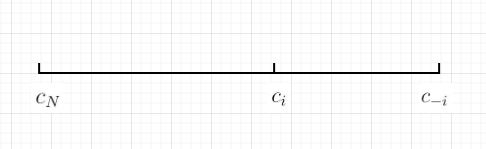
\includegraphics[width=0.61\textwidth]{Chapter-2/Figures/cncic-i.JPG}}
%   \subfigure[]{
%     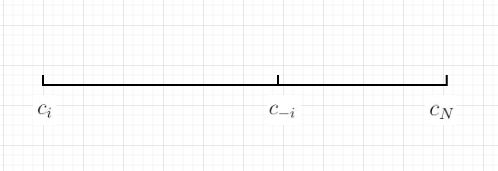
\includegraphics[width=0.61\textwidth]{Chapter-2/Figures/cic-icn.JPG}}
%   \caption{When $c_N$ lies outside the range of $c_i$ and $c_{-i}$}
%   \label{cnci}
% \end{figure}

Whether Equation \ref{unjpgt} exceeds 1 is determined by the relative values of $c_i$ and $c_N$ and national government's provision in $i$.

I constructed a one-dimensional line segment to depict the relationship between $c_i$ and $c_N$. The calculation of Equation \ref{unjpgt} is straightforward  when the relationship are illustrated in Figure \ref{cnci}. In the depicted relationship, represented by subfigure $(a)$ in Figure \ref{cnci}, $\frac{c_l\cdot G_{Nl}+c_h\cdot G_{Nh}}{c_N\cdot (G_{Nl}+G_{Nh})}>1$, prompting the national government to prefer joint provision over general transfer, and vice versa.

% \begin{figure}[htbp]
%   \centering
%   \subfigure[]{
%     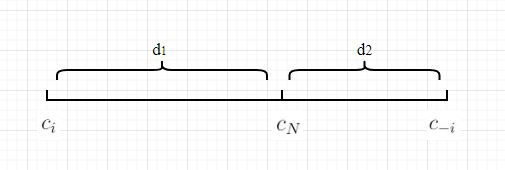
\includegraphics[width=0.71\textwidth]{Chapter-2/Figures/cicnc-i.JPG}}
%   \subfigure[]{
%     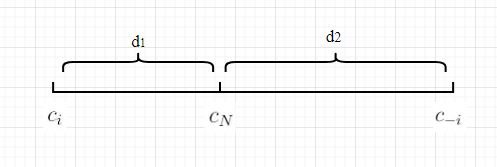
\includegraphics[width=0.71\textwidth]{Chapter-2/Figures/cicnc-i2.JPG}}
%   \caption{When $c_N$ lies between $c_i$ and $c_i$}
%   \label{cnci2}
% \end{figure}

When price for public goods by national government lies between $c_i$ and $c_{-i}$ shown in figure \ref{cnci2} \footnote{$c_{-i}$ is the price of $S_{-i}$, which is the one that is not $i$ among the two. }.

I define the distance between $c_i$ and $c_N$ as $d_1$ and distance between $c_{-i}$ and $c_N$ as $d_2$. Thus I have

$$
    \left\{\begin{array}{l}
        C_i=C_N-d_i \\
        C_{-i}=C_N+d_2
    \end{array}\right.
$$
Equation \ref{unjpgt} can be rewritten as:

\begin{equation}
    1+(G_{Nh} \cdot d_2-G_{Nl} \cdot d_1) \label{unjpgt2}
\end{equation}

I define $$G_{Nl}= a \cdot G_{Nh}$$ to represent national government's provision distribution where a capture the relationship between $G_{Nl}$ and $G_{Nh}$. Equation \ref{unjpgt2} can be rewritten as:

\begin{equation}
    1+G_{Nl}(a \cdot d_2-d_1) \label{unjpgt3}
\end{equation}


Equation \ref{unjpgt2} implies that when $c_N$ is situated between $c_i$ and $c_{-i}$, the national government's decision between general transfers and joint provision is determined by $(a \cdot d_2 - d_1)$. This implies that the national government aims to equalize public goods across subnational jurisdictions with minimal tax burden, demonstrating its concern for both $c_l$ and $c_h$. Under certain circumstances, especially when one jurisdiction faces a significantly higher public goods price, such that $\frac{d_1}{d_2}<a$ (indicated by a large $d_2$).%%%chatgpt checked%%%%%

\begin {itemize}
\item \textbf{Proposition 6: The subnational governments aligned with national government are more likely to accept the categorical transfer.}
\end{itemize}

The condition for subnational governments to accept the categorical transfer is $U^*_i|_{CT}>U^*_i|_{NP}$, which can be rewritten as:

\begin{equation}
    \frac{\alpha_i^2 e_i^2 F_i^2}{4c_i^2|_{CT}}-\frac{\alpha_i^2 e_i^2 F_i^2}{4c_i^2|_{NP}}> \gamma_i|X_N-X_i|
\end{equation}

Aligned governments imply shared policy preferences between national and subnational governments. In extreme circumstances, when the national government precisely aligns with subnational governments in their ideal policy positions ($X_N = X_i$), policy deviation becomes zero. Beyond the policy preference gap between national and subnational governments, alignment with the national government may result in preferential treatment for subnational governments during national decision-making. This, in turn, leads to increased tolerance for policy deviation in categorical transfer games (a smaller $\gamma_i$). %%%chatgpt checked%%%%%


\section{Explain of Fiscal Phenomenon during Intergovernmental Transfer}

This paper contributes to the explanation of fiscal phenomena from two perspectives. Firstly, it explores the impact of intergovernmental transfers on subnational spending, encompassing the flypaper effect and fungibility effect. Another area of interest pertains to understanding the dominance of categorical transfers in intergovernmental fiscal arrangements.%%chatgpt checked%%%%%

\subsection{Flypaper Effect and Fungibility Effect}


As mentioned in the literature regarding the impact of intergovernmental transfers on subnational spending, researchers have found empirical evidence supporting contradictory theories—the flypaper effect and the fungibility effect. While there is substantial evidence supporting the flypaper effect, empirical support for fungibility is comparatively limited \parencite{zampelli1986resource, khilji1991fungibility, khilji1994fungibility}. The model I have constructed aims to elucidate the flypaper effect by addressing two key questions: firstly, why does the flypaper effect exist? And secondly, why do contradictory conclusions exist, with limited supportive evidence for fungibility?%%chatgpt checked%%%%%

The flypaper effect of categorical transfers is intuitively reasonable and widely accepted by scholars, as it lowers costs. Therefore, the critical aspect is to explain the flypaper effect of general transfers.%%chatgpt checked%%%%%

In the game theory model, the contradiction of general transfer can be explained by equation \ref{gofgeneral}.

$$G_i^*|_{GT}=\frac{\alpha_i e_i^2F_i^2}{2c_i^2}+\frac{T_i}{c_i}-\frac{1}{2}\cdot \frac{e_i}{e_N}\cdot \frac{F_i}{\sum F_i} \cdot \frac{\sum T_i}{c_i}$$

Empirical evidence supports both the flypaper effect and the fungibility effect, as demonstrated by the comparison between $\frac{T_i}{c_i}$ and $\frac{1}{2}\cdot \frac{e_i}{e_N}\cdot \frac{F_i}{\sum F_i} \cdot \frac{\sum T_i}{c_i}$. The first term, $\frac{\alpha_i e_i^2F_i^2}{2c_i^2}$, represents local public goods provision without external disturbances. The term $\frac{T_i}{c_i}$ reflects the flypaper effect, indicating an increase in provision resulting from general transfers. On the other hand, the term $\frac{1}{2}\cdot \frac{e_i}{e_N}\cdot \frac{F_i}{\sum F_i} \cdot \frac{\sum T_i}{c_i}$ encapsulates the fungibility effect, signifying a decrease in provision due to general transfers. The comparison between the flypaper effect term and the fungibility effect terms can be expressed as follows:%%chatgpt checked%%%%%

\begin{equation}
    T_i-\frac{1}{2}\cdot \frac{e_i}{e_N}\cdot \frac{F_i}{\sum F_i} \cdot \sum T_i \label{compare}
\end{equation}


This equation provides an explanation for the coexistence of contradictory theories—the flypaper effect and fungibility—and sheds light on the limited empirical evidence regarding fungibility. When $T_i>\frac{1}{2}\cdot \frac{e_i}{e_N}\cdot \frac{F_i}{\sum F_i} \cdot \sum T_i$, the flypaper effect prevails. Conversely, if $T_i<\frac{1}{2}\cdot \frac{e_i}{e_N}\cdot \frac{F_i}{\sum F_i} \cdot \sum T_i$, fungibility dominates.

Why evidence of the fungibility effect is relatively scarce remains a question. Building on the analysis of Equation \ref{compare}, I propose explanations for the prevalence of the flypaper effect, as outlined in Propositions 7 and 8.

\begin {itemize}
\item \textbf{Proposition 7: One factor contributing to the flypaper effect is citizens' aversion to taxes.}
\end{itemize}

One factor contributing to $T_i>\frac{1}{2}\cdot \frac{e_i}{e_N}\cdot \frac{F_i}{\sum F_i} \cdot \sum T_i$ is the presence of the parameter $\frac{1}{2}$. This parameter arises from citizens' aversion to tax collection\footnote{I adopt the square form for tax burden solely for computational convenience in this specific case. Nevertheless, as long as aversion exists, the exponent of the tax burden should exceed 1, resulting in a parameter less than 1.}. Tax aversion for subnational governments implies that increasing taxes is prohibitively costly, a phenomenon known as the distortion effect of tax increases. This concept aligns with several existing studies explaining the flypaper effect. \Textcite{hamilton1986flypaper} was the first to observe that the cost of tax collection within a jurisdiction results in a distortionary tax. \Textcite{dahlby2016stimulative} argued that the non-matching grants create a price effect, attributable to subnational governments' information and ability disadvantages. \Textcite{vegh2016unsticking} arrived at a similar conclusion.%%chatgpt checked%%%%%

Horizontal government interactions further elucidate this distortion. \Textcite{brueckner2003strategic} concludes that lower-level governments are highly sensitive to actions taken by their counterparts, potentially explaining the reluctance of state and local governments to increase taxes for public goods. Other theories of horizontal interaction, such as yardstick competition or tax competition, also contribute to understanding this sensitivity \parencite{shleifer1985theory,revelli2006performance}.%%chatgpt checked%%%%%

\begin {itemize}
\item \textbf{Proposition 8: Subnational governments with varying resource endowments exhibit different magnitudes of the flypaper effect.}
\end{itemize}

The fungibility effect is adjusted by two factors $\frac{F_i}{\sum_i F_i}$ and $\frac{e_i}{e_N}$. For $S_l$, $\frac{F_l}{\sum_i F_i}$ could be a small value, which would lead to $T_l-\frac{1}{2}\cdot \frac{e_l}{e_N}\cdot \frac{F_l}{\sum F_i} \cdot \sum T_i>0$.

In the context of tax collection efficiency, the literature generally concurs that tax collection efficiency is positively associated with the level of economic development \parencite{arvate2008efficiency,mattos2011flypaper}. Regions with lower economic output, denoted as $S_l$, typically experience reduced tax collection efficiency. This disparity amplifies the gap between $T_l$ and $\frac{1}{2}\cdot \frac{e_l}{e_N}\cdot \frac{F_l}{\sum F_i} \cdot \sum T_i$, thereby leading to a larger magnitude of the flypaper effect, vice versa.%%chatgpt checked%%%

An implication drawn from Proposition 8 is that, in entities with imbalanced regional development, underdeveloped regions may exhibit a greater tendency to increase spending upon receiving general transfers. Bowman's 1974 research, using federal education grants to West Virginia as an example to measure the scale of the flypaper effect, found that a one-dollar increase in governmental transfers to school districts resulted in 1.06 times more spending compared to the same increase in tax revenue \parencite{bowman1974tax}. In contrast, Weicher's evaluation of the flypaper effect suggested that state grants to school districts in America, on average, led to 0.4 times more spending \parencite{weicher1972aid}. Despite both investigations being conducted around the same time and addressing the same topic— the scale of the flypaper effect in school districts—the observed scales differed significantly. One possible explanation for this discrepancy is that West Virginia ranked 48th in GDP.%%chatgpt checked%%%

\begin{itemize}
    \item \textbf{Proposition 9: One potential reason for the flypaper effect empirical evidence in $S_l$ is the relatively disadvantage in tax collection efficiency compared to national government.}
\end{itemize}

Literature on tax collection efficiency generally share a consent that tax collection efficiency positively related with the economic development level \parencite{arvate2008efficiency,mattos2011flypaper}. A region with low economic output $S_l$ typically leads to lower tax collection efficiency, which enlarge the gap between $T_l$ and $\frac{1}{2}\cdot \frac{e_l}{e_N}\cdot \frac{F_l}{\sum F_i} \cdot \sum T_i$, which leads to greater size of flypaper effect. Combined proposition 8 with proposition 9, one deduction is: for those economy entity with imbalanced regional development, those underdeveloped regions may show greater spending tendency when receiving general transfer. In Bowman's research conducted in 1974, he use federal education grants to West Virginia as example to measure flypaper effect scale \parencite{bowman1974tax}. His conclusion is that one dollar increase in governmental transfer to school districts would lead to 1.06 more spending compared to the same increase in tax revenue. As a contrast, Weicher also evaluates the size of flypaper effect and conclude that the states grants to school districts in America would lead to 0.4 more spending on average \parencite{weicher1972aid}. These two investigation were generated in roughly same time and discuss same topics: scale of flypaper effect in school districts. However the scale differ greatly. One explanation is: West Virginia ranks 48th in GDP.

\begin{itemize}
    \item \textbf{Proposition 10: One potential reason for the flypaper effect empirical evidence in $S_h$ is citizen's tax aversion.}
\end{itemize}

One natural following question after proposition 8 and 9 is: how could flypaper effect evidence is also wildly found in high economic output region, such as some empirical research conducted in California, New York and some developed states in India \parencite{nguyen2020flypaper,bae2004flypaper,lalvani2002flypaper}. The explain is the constant parameter in $\frac{1}{2}\cdot \frac{e_l}{e_N}\cdot \frac{F_l}{\sum F_i} \cdot \sum T_i$, which is 1 and $\frac{1}{2}$ here. The difference between the parameter is due to citizen's concave or linear utility on public goods increase and convex tax burden increase.\footnote{In my utility setting, the utility for public goods is set as linear to get arithmetic expression, the actual utility maybe concave but this won't change the conclusion here.} In other words, citizen gets inertia as public goods increase and sensitive as tax burden increase. So, the general transfer naturally stimulate local governments' spending.

Under what circumstances would regional's choice on public spending shows fungibility? From equation \ref*{compare}, we can have a basic image about the jurisdiction that shows fungibility effect to intergovernmental transfer: a region with higher output percentage in total output, higher tax collection efficiency compared to national government, lacking feeling about tax increase.
\subsection{The Overwhelming Weight of Categorical Transfer}

One necessary but insufficient condition for the national government to propose a categorical transfer is $U_N|_{CT} > U_N|_{NP}$, which can be rewritten as:

\begin{equation}
    \sum_i(\frac{\alpha_i^2e_i^2F_i^2}{2c_i^2|_{CT}}-\frac{\alpha_i^2e_i^2F_i^2}{2c_i^2|_{NP}}) +\sum_i\gamma_i|X_i-y_i|>\delta D \label{6666}
\end{equation}

The prevalence of categorical transfers can be partly explained by the right side of Equation \ref{6666}. When issued bonds mature over an extended period, or when the national government prioritizes immediate benefits at the expense of future generations' debt burden, categorical transfers become a valuable tool as they alleviate the tax burden. In other words, this represents a trade-off between long-term and short-term utility.

\section{Review and Summary}

In this paper, I aim to elucidate the decision-making process of fiscal policy in public goods provision through the interaction of national and subnational governments. The impact of the joint efforts of national governments on public goods provision, specifically whether it leads to a 'squeeze in' or 'squeeze out' effect on the quantity of public goods in subnational jurisdiction $S_i$, is influenced by various parameters. %%chatgpt checked%%%

In summary, the key question for subnational governments is whether to accept a categorical transfer once the method is chosen, and the matching ratio is determined by the national government. This decision hinges on the comparison between the utility for subnational governments in a non-provision game and a categorical transfer game. The evaluation for subnational governments involves a trade-off between policy inutility and a lower price. The decision on categorical transfer is the only one jointly made by the national and subnational governments. While rejecting the joint provision or general transfer is not in violation of any rules, subnational governments lack motivation to do so. The rationale is that regardless of whether a subnational government rejects a categorical transfer or joint provision offer, taxes from the national government are imposed on the entire nation. Therefore, accepting the general transfer or joint provision offer would at least prevent the imposition of taxes in vain. %%chatgpt checked%%%

The national government evaluates utility based on the subnational government's level of public goods provision, denoted as $G_i^*$. The adoption of categorical transfer represents a joint decision by both the national and subnational governments. If the subnational government is satisfied with the categorical transfer offer and it proves to be the optimal choice for the national government among all subgames, then the categorical transfer is implemented.

Compared to Volden's framework, I modified the utility settings and introduced the categorical transfer into the analysis. However, in examining the impact of categorical transfer, the comparison between different games does not yield a straightforward arithmetic solution, representing a limitation in contrast to Volden's original setup.%%chatgpt checked%%%

One distinct conclusion from the modified model, when compared to the propositions in \Textcite{volden2007intergovernmental}'s paper, is that the competition effect between the national government and subnational government in providing goods is not as significant; instead, the free rider effect dominates. Consequently, rejecting grants is more likely due to policy outcome deviation and dissatisfaction with the grant scale, rather than stemming from provision competition. Meanwhile, both levels of government are sensitive to tax increases.%%chatgpt checked%%%

Another debatable issue involves the national government's funding mechanism for supporting categorical transfers. In contrast to general transfers and joint provision, the national government in this scenario opts for bond issuance to finance categorical grants rather than relying on taxes. This change introduces ambiguity when evaluating the national government's choice between categorical transfer and other games. Despite this apparent drawback, the setting is reasonable for two main reasons. Firstly, many categorical transfer programs, especially in American and OECD countries, commonly rely on bonds for support \parencite{spahn2012conditioning,de2007local,weist2007intergovernmental}. Secondly, categorical transfer and general transfer serve distinct purposes for the national government. Categorical transfer aims to stimulate spending in specific areas, while general transfer and joint provision seek to equalize public goods spending across different jurisdictions. Consequently, comparing categorical transfer and general transfer within the same framework is unreasonable.%%chatgpt checked%%%

While I acknowledge that this theoretical inference for fiscal interaction is far from complete, it is impractical to include every possible factor in the model. For instance, \Textcite{nicholson2012leaving} indicates that subnational governments controlled by different parties exhibit distinct attitudes toward grants. Political factors such as whether the governor is an incumbent or facing an election also play a significant role \parencite{nordhaus1975political, macrae1977political}. This paper just provides a general framework for understanding the cognitive mechanisms in governmental joint decision-making and interaction behavior regarding intergovernmental transfers.

Furthermore, empirical evidence is essential to validate the propositions presented in this paper. For certain propositions, well-designed empirical tools are imperative. For instance, I posit that the competition effect is rare, and the refuse of categorical transfers is more likely attributable to policy outcome deviation. In the empirical process, distinguishing whether subnational governments reject grants due to provision competition or policy deviation poses a challenge, as we can only observe behavior, not motivations. Thus, a properly designed empirical test is crucial for future research.